%!TEX root = syntheyes15.tex

\section{Synthetic data generation}

In this section we first present our anatomically inspired CG eyeball model, and then explain our novel procedure for preparing a suite of 3D head scans for dynamic photorealistic labelled data generation. We then briefly describe how we use image-based lighting \cite{debevec2002image} to model a wide range of realistic lighting conditions, and finally discuss the details of our rendering setup.

% \cite{MIL-STD-1472G} -- cite for range of eye rotation.

\subsection{Eye model}

\begin{figure}
    \centering
    \begin{subfigure}[t]{0.33\columnwidth}
        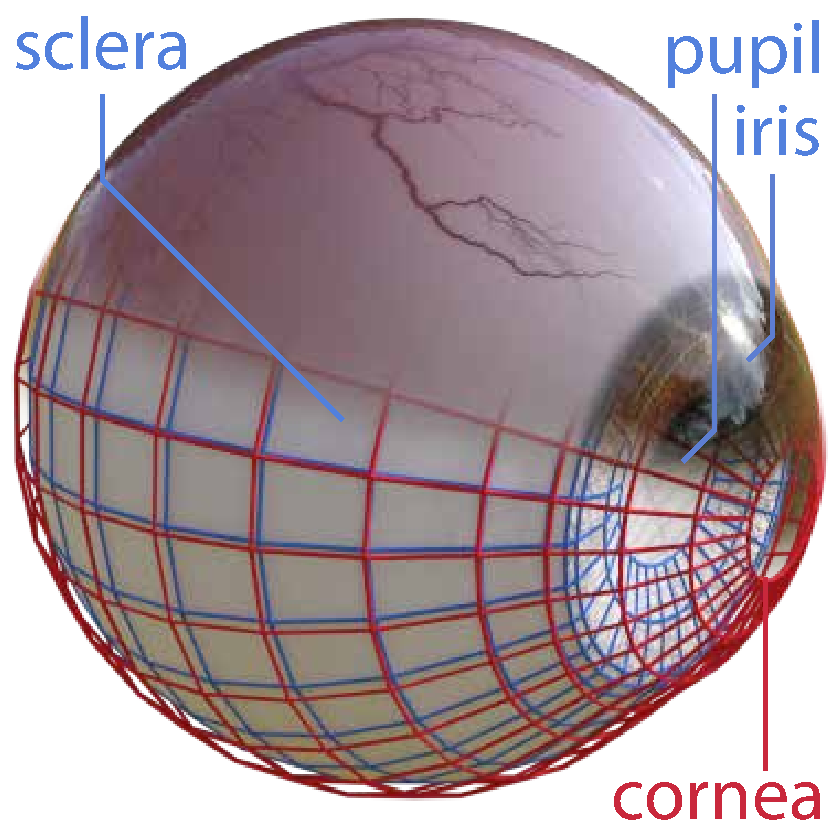
\includegraphics[width=\textwidth]{eye_model}
        \caption{3D eye model}
        \label{fig:3d_eye_model}
    \end{subfigure}%
    \hfill
    \begin{subfigure}[t]{0.65\columnwidth}
        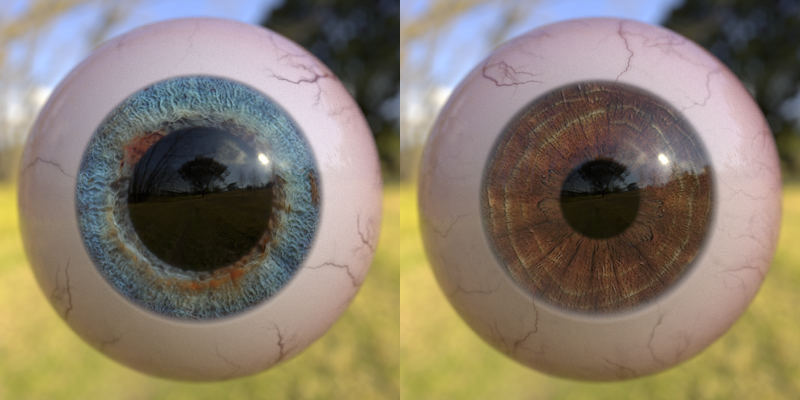
\includegraphics[width=\textwidth]{eye_examples}
        \caption{Pupil dilation and iris color variation}
    \end{subfigure}
    \caption{Our realistic eye model is capable of expressing degrees of variability seen in real life.}
    \label{fig:eye_model}
\end{figure}

Eyeballs are complex organs comprised of multiple layers of tissue, each with different reflectance properties and levels of transparency. Fortunately, as realistic eyes are so important for many areas of CG, there is already a large body of previous work on modelling and rendering eyes \commentE{cite}.

% It is important to accurately model reflections and refractions in the eye as they can lead to specular highlights -- these common eye-region image features are often used by eye-tracking algorithms, or can confound approaches that are not robust.

As shown in \autoref{fig:3d_eye_model}, our eye model consists of two parts.
%
The outer part (red wireframe) approximates the eye's overall shape with two spheres ($r_1\!=\!12\textrm{mm}, r_2\!=\!8\textrm{mm}$ \cite{ruhland2014look}), the latter representing the corneal bulge. To avoid a discontinuous seam between spheres, the meshes were joined and then smoothed. It is transparent, refractive ($n\!=\!1.376$), and partially reflective. The eye's bumpy surface variation is modelled by a displacement map generated with noise functions.
%
The inner part (blue wireframe) is a flattened sphere with Lambertian material. The planar end represents the iris and pupil, and the rest represents the sclera -- the white of the eye.
%
There is a $0.5\textrm{mm}$ gap between the outer and inner parts which accounts for the thickness of the cornea. \commentE{compare with recent Disney work}

Eyes exhibit variations in both shape (pupillary dilation) and texture (iris color and scleral veins). To model shape variation we use \emph{shape keys} -- a CG animation technique where different versions of a mesh are stored, modified, and interpolated between. We have shape keys for dilated and constricted pupils, as well as large and small irises to account for a small amount ($10\%$) of iris size variation.

We vary the appearance of the eye by compositing textures in three separate layers:
\begin{inparaenum}[\itshape i\upshape)]
\item a \emph{sclera} layer representing the tint of the sclera (white, pink, or yellow);
\item an \emph{iris} layer with four photo-textures of different colored irises (amber, blue, brown, grey); and
\item a \emph{veins} layer which varies between blood-shot and clear
\end{inparaenum}. We matched the sclera tint to each separate face model, but uniformably randomly varied iris color. Previous research on iris-synthesis \commentE{cite} would have allowed continually different iris textures, but we decided this added complexity would not make a worthwhile improvement in overall appearance variation, especially when rendered at lower resolutions.

\subsection{Preparing a suite of 3D eye-region models}

\begin{figure}
    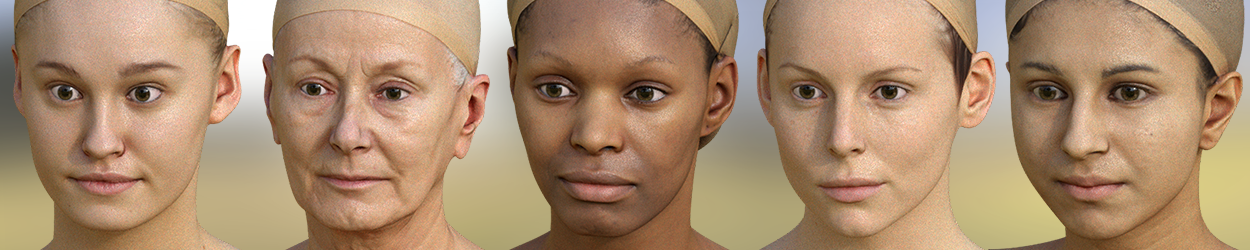
\includegraphics[width=\columnwidth]{participants_f} \par \smallskip
    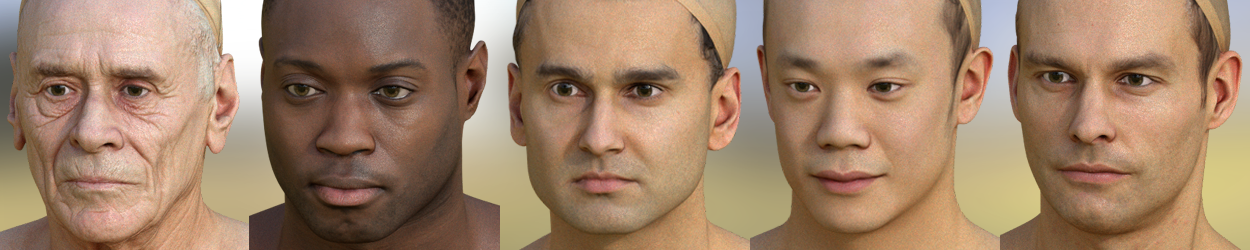
\includegraphics[width=\columnwidth]{participants_m}
    \caption{Our suite of female and male head models for rendering.}
    \label{fig:participants}
\end{figure}

Remove scanned eye. 

\subsubsection{Eyelid motion}

Vertical saccades are always accompanied by eyelid motion \cite{liversedge2011oxford}.

\subsection{Lighting}

\begin{figure}
    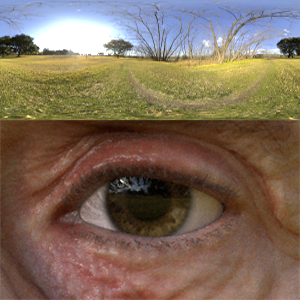
\includegraphics[width=0.24\columnwidth]{fig_env_1} \hfill
    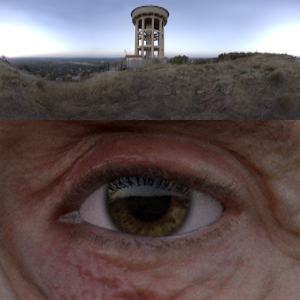
\includegraphics[width=0.24\columnwidth]{fig_env_2} \hfill
    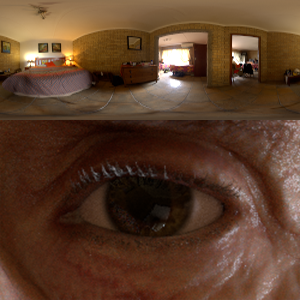
\includegraphics[width=0.24\columnwidth]{fig_env_3} \hfill
    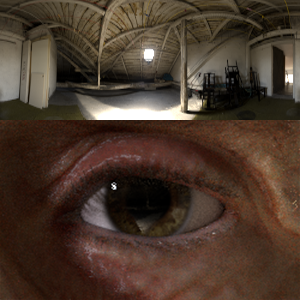
\includegraphics[width=0.24\columnwidth]{fig_env_4}
    \caption{Appearance variation from lighting is modelled with poseable high-dynamic-range environment maps \cite{debevec2002image}.}
    \label{fig:participants}
\end{figure}
